\documentclass[12pt]{article}
\usepackage{amsmath}
\usepackage{enumitem}
\usepackage{graphicx}
\usepackage{float}

\newlist{subquestion}{enumerate}{1}
\setlist[subquestion,1]{label=(\alph*)}
\setlength{\parindent}{4cm}

\begin{document}

\title{CS 430 Homework 3}
\author{Sarah Kushner}
\date{\today}
\maketitle

\begin{enumerate}

\item 
\textbf{C$^0$} \\
Two curves are $C^i$ continuous at point $p$ iff the $i^{th}$ derivative of the curves are equal at $p$.
When two curves are $C^0$ continuous, there is a discontinuity in the slope. Their first derivatives are not equal.

(Note: I made the drawings with Google Drawings.) \\
\begin{figure}[H]
    \centering
	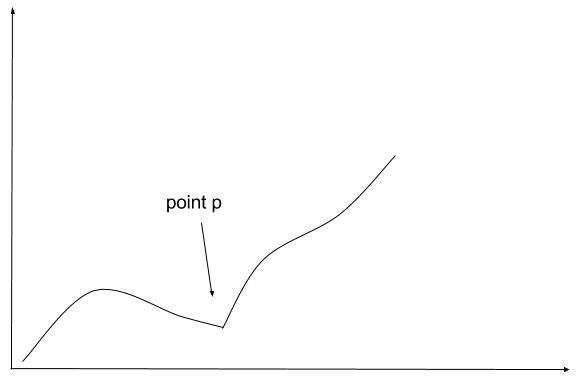
\includegraphics[width=0.4\textwidth]{C0}
    \caption{$C^0$ continuity.}
\end{figure}

\item 
\textbf{C$^1$} \\
When two curves are $C^1$ continuous, there is a discontinuity in the curvature. Their first derivatives are equal, but their second derivatives are not.

\begin{figure}[H]
    \centering
	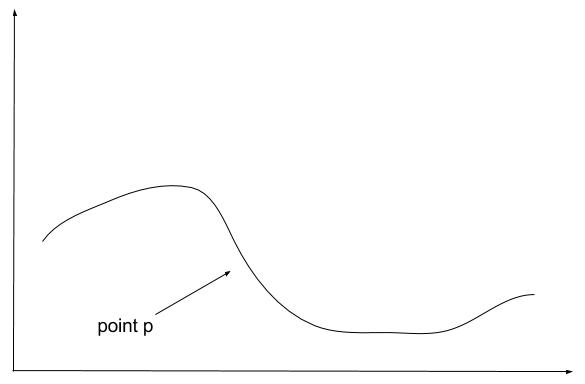
\includegraphics[width=0.4\textwidth]{C1}
    \caption{$C^1$ continuity.}
\end{figure}

\item 
\textbf{C$^2$} \\
When two curves are $C^2$ continuous, their first and second derivatives are both equal.

\begin{figure}[H]
    \centering
	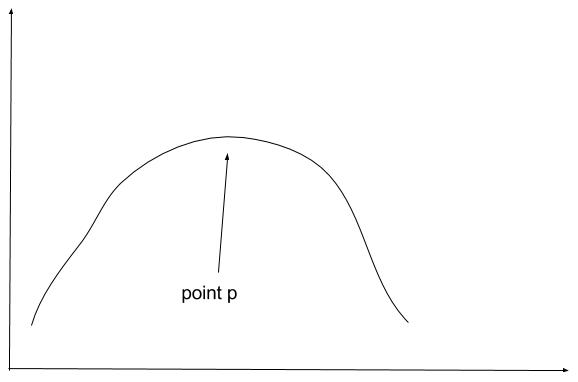
\includegraphics[width=0.4\textwidth]{C2}
    \caption{$C^2$ continuity.}
\end{figure}

\item
\textbf{True or False} \\
\begin{subquestion}
\item
False. The number of control points is independent of the degree of the B-spline curve.

\item 
True. B-splines have a local control property which means each control point affects its local curve.

\item 
True. Using non-uniform B-splines, they can be forced to interpolate their control points.

\item
False. B-splines are single piecewise curves.

\end{subquestion}

\pagebreak

\item  
\textbf{Bernstein Polynomials} \\
The basis matrix of a B\'ezier curve with 3 control points and using polynomials of degree 2 \\ \\
$b_{02} = \binom{2}{0} (1-t)^2 t^0 = (1-t)^2 = t^2 - 2t +1$ \\
$b_{12} = \binom{2}{1} (1-t)^1 t^1 = 2(1-t)t = -2t^2 + 2t $ \\
$b_{22} = \binom{2}{2} (1-t)^0 t^2 = (1-t)^0 t^2 = t^2$ \\

\[
\begin{bmatrix}
    1  & -2 & 1 \\
    -2 & 2  & 0 \\
    1  & 0  & 0
\end{bmatrix}
\]

\item
\textbf{B\'ezier Curve} \\
\begin{subquestion}
\item
G = $
\begin{bmatrix}
    2  & 4  & 5 & 0 \\
    4  & 2  & 7 & 0 \\
\end{bmatrix}
$

\item 
M = $
\begin{bmatrix}
    -1  & 3   & -3 & 1 \\
    3   & -6  & 3  & 0 \\
    -3  & 3   & 0  & 0 \\
    1   & 0   & 0  & 0 \\
\end{bmatrix}
$

\item 
Q = GMT \\
GM = $
\begin{bmatrix}
    -5   & -3  & 6  & 2 \\
    -19  & 21  & -6 & 4 \\
\end{bmatrix}
$ \\
T = $
\begin{bmatrix}
	 t^3  \\
     t^2  \\
     t   \\
     1   \\
\end{bmatrix}
$ \\
Q = $
\begin{bmatrix}
	 -5t^3-3t^2+6t+2  \\
     -19t^3+21t^2-6t+4  \\
\end{bmatrix}
$

\item
Q$(0.5)$ = (3.625, 3.875) \\

\end{subquestion}

\pagebreak

\item
\textbf{de Casteljau} \\
$p_{00} = (2,4)$ \\
$p_{10} = (4,2)$ \\
$p_{20} = (5,7)$ \\
$p_{30} = (0,0)$ \\

r = 1 \\
$p_{01}(u)$ \\ 
$= (1-u)(2,4)+u(4,2) = (2-2u,4-4u) + (4u,2u)$ \\ 
$= (2+2u,4-2u)$ \\

$p_{11}(u)$ \\ 
$= (1-u)(4,2)+u(5,7) = (4-4u,2-2u) + (5u,7u)$ \\ 
$= (4+u,2-5u)$ \\

$p_{21}(u) = (1-u)(5,7)+u(0,0) = (5-5u,7-7u)$ \\

r = 2 \\
$p_{02}(u) $ \\
$= (1-u)(2+2u,4-2u)+u(4+u,2-5u)$ \\
$= (-2u^2+2,2u^2-6u+4) + (4u+u^2,2u+5u^2)$ \\
$= (-u^2+4u+2,7u^2-4u+4)$ \\

$p_{12}(u) $ \\
$= (1-u)(4+u,2-5u)+u(5-5u,7-7u)$ \\
$= (4-3u-u^2,2+3u-5u^2) + (5u-5^2,7u-7u^2)$ \\
$= (-6u^2+2u+4,-12u^2-10u+2)$ \\

r = 3 \\
$p_{03}(u) $ \\
$= (1-u)(-u^2+4u+2,7u^2-4u+4)+u(-6u^2+2u+4,-12u^2-10u+2)$ \\
$= (u^3-5u^2+2u+2,-7u^3+11u^2-8u+4) + (-6u^3+2u^2+4u,-12u^3+10u^2+2u)$ \\
$= (-5u^3-3u^2+6u+2,-19u^3+21u^2-6u+4)$ \\

$u = 0.5$ \\

(3.625, 3.875) \\

\end{enumerate}

\end{document}